\chapter{Dataontwerp}

\begin{figure}[h!]
	\centering
		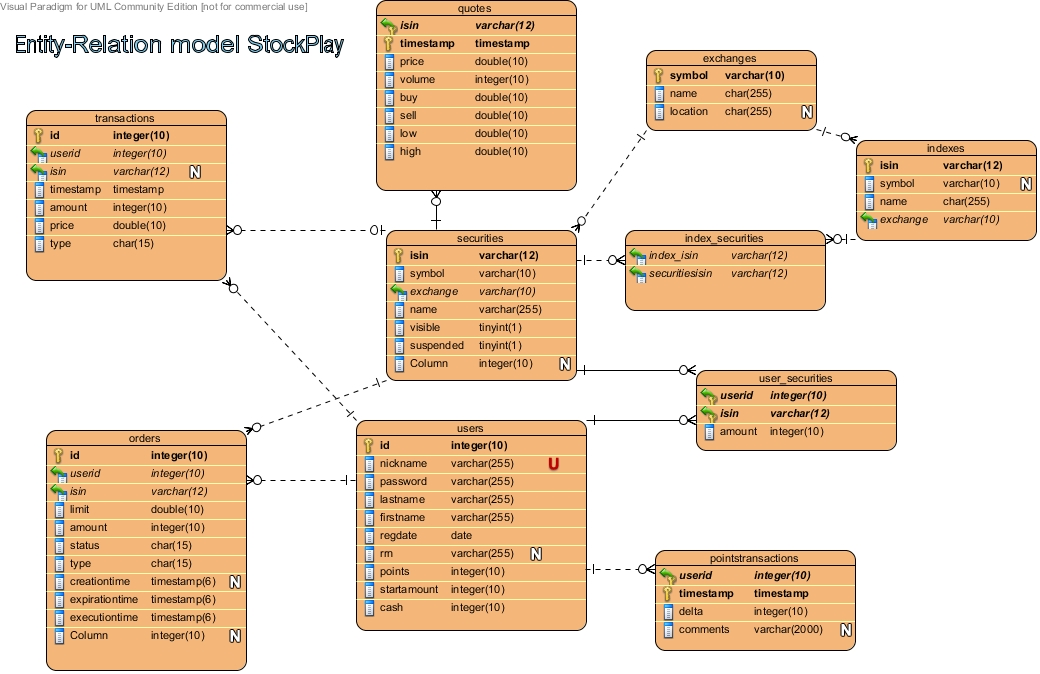
\includegraphics[width=0.5\textwidth]{images/realisatie/ER_Diagram}
	\caption{Entity-relationship model.}
\end{figure}

\section{Ontwerp backend}
\todo{dit hoort hier niet}
De klassen die de persistente data uit de database moeten weergeven staan opgesomd in onderstaand klassendiagram:

\begin{figure}[h!]
	\centering
		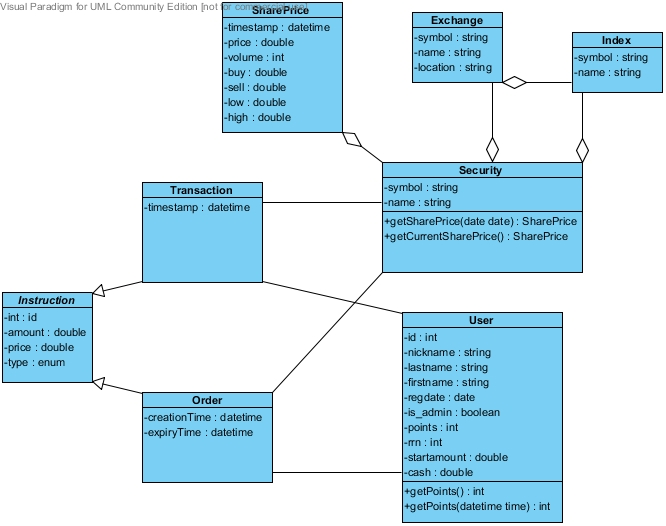
\includegraphics[width=0.5\textwidth]{images/realisatie/Class_Diagram}
	\caption{Klassendiagram persistente data in backend.}
\end{figure}

\chapter{Procedureontwerp}

\section{Backend protocol}

Alle databasetoegang wordt uitgevoerd via een gemeenschappelijke backend. Hiervoor hebben we een interface opgesteld volgens een aantal richtlijnen:
\begin{itemize}
\item{taalonafhankelijk: aangezien de interfaces met behulp van verschillende programmeertalen gerealiseerd worden, moet de interface toegankelijk zijn vanuit verschillende programmeertalen.}
\item{lichtgewicht: voor de communcicatie met onze mobiele interface, moet de gegenereerde data compact gehouden worden.}
\item{toegankelijk: de interfaces moeten toegankelijk zijn vanaf een andere machine dan die waar de backand op draait.}
\end{itemize}

Voor de interface met de backand hebben we een aantal interfaces overwogen:

\begin{itemize}
\item{een eigen binair protocol}
\item{SOAP API}
\item{XML-RPC}
\item{RMI}
\end{itemize}

We hebben uiteindelijk gekozen voor het XML-RPC protocol. Dit is een lichtgewicht Remote Procedure protocol, die methodeaanvragen en -antwoorden verpakt in XML-data en ze als POST request verstuurd over het HTTP protocol (zie ook bijlage \ref{chap:xml-rpc} voor de specificaties).

Voor het binair protocol hebben we niet gekozen om dat we hiervoor een stuk meer zouden moeten implementeren. Alsook werkt dit niet over het HTTP protocol, zodat dit eventueel op bepaalde netwerken geblokkeerd zou kunnen worden. Een SOAP API zou een stuk zwaarder uitvallen dan XML-RPC en RMI is enkel niet taalonafhankelijk. 

Het XML-RPC protocol voldoet aan de opgestelde eisen: aangezien het verder =bouwt op het bestaande HTTP-protocol kan het gebruik maken van diens mogelijkheden (zoals compressie en encryptie) en kan het indien een specifieke bibliotheek onbestaande is eenvoudig verwerkt worden via reeds bestaande HTTP- en XML-bibliotheken. Bovendien verschilt de communicatie niet van regulier http verkeerd waardoor de toegankelijkheid in gelimiteerde netwerkomgevingen ook toeneemt.

Voor de programmeertalen die we gaan gebruiken bij het implementeren blijken er reeds verschillende bibliotheken beschikbaar te zijn, wat het gemak van gebruik opnieuw verhoogt. Een opsomming van de specifieke bibliotheken die we zullen gebruiken om informatie te versturen en ontvangen over het XML-RPC protocol:
\begin{itemize}
\item{\textbf{Perl}: \makeurl{XML::RPC}{http://search.cpan.org/~daan/XML-RPC-0.9/lib/XML/RPC.pm}}
\item{\textbf{C\#}: \makeurl{XML-RPC.NET}{http://www.xml-rpc.net/}}
\item{\textbf{Java}: \makeurl{Apache XML-RPC}{http://ws.apache.org/xmlrpc/}}
\end{itemize}

\todo{XML, Redstone en Marque}

Aangezien XML-RPC geen ondersteuning biedt voor namespaces of andere vormen van functieorganisatie, hanteren we zelf een mechanisme om dit te bekomen: een methode-naam bestaat altijd uit twee delen, gescheiden door een punt. Het deel voor het scheidingsteken duidt het pakket aan, het deel erna de methode die we willen oproepen.
Zo delen we de backend op in de volgende drie primaire klassen:
\begin{itemize}
\item{System: functionaliteit voor beheer en de statusinformatie van het systeem.}
\item{User: beheer van gebruikers en ophalen gebruikersinformatie.}
\item{Finance: functionaliteit gerelateerd aan het beurswezen.}
\end{itemize}
Hogere-orde klassen zijn eventueel ook mogelijk (zoals \emph{System.Database}), maar niet verplicht. De semantiek is daarbij identiek aan primaire klassen, met een punt als scheidingsteken.

\subsection{Algemene foutcodes}

De XML-RPC specificatie biedt ook ondersteuning voor foutberichten, in de form van een bericht met een $<$fault$>$ tag. Die tag moet steeds twee $<$member$>$ tags bevatten, namelijk een foutcode $<$faultCode$>$ van het integer type, en een foutbericht $<$faultString$>$ van het string type. Elk van de klassen kan zo specifieke foutmeldingen vastleggen.
Maar er zijn ook generieke foutmeldingen, die van toepassing zijn op alle klassen. Deze foutmeldingen, waarvan de foutcode in het bereik $[0, 100[$ valt, worden hieronder beschreven:

\begin{table}
\begin{tabular}{| c p{5cm} p{7cm} |}
	\hline
	Foutcode & Foutbericht & Controle \\
	\hline
	
	0 & Internal Failure & Verifieer de status van de backend, de log kan hierbij helpen. \\
	\hline
	
	$[1-10[$ & \emph{Subsystem failures.} & \\
	1 & Database Failure & Er is een probleem met de database (onbeschikbaar, corrupt, ...), zie de log voor meer details. \\
	2 & Scraper Failure & Er is een probleem met de scraper (onbeschikbaar, uitgevallen, ...), zie de log voor meer details. \\
	\hline
	
	$[10-20[$ & \emph{Service issues.} & \\
	10 & Service Unavailable & De backend kan tijdelijk niet gebruikt worden (werkzaamheden, overloaded, ...). \\
	11 & Unauthorized & Meld u aan vooraleer deze functie te gebruiken. \\
	\hline
	
	$[20-30[$ & \emph{Invocation issues.} & \\
	20 & Version Not Supported & De client gebruikt een verkeerd communicatieprotocol. \\
	21 & Not Found & Methode niet gevonden, verifieer de schrijfwijze en de klasse. \\
	21 & Bad Request & Probleem met de parameters, controleer het gebruik van de methode. \\
	\hline
\end{tabular}
\caption{Generieke foutcodes in het backend-protocol.}
\end{table}

\subsection{Authenticatie en autorisatie}

Aangezien het XML-RPC protocol gebruik maakt van het HTTP-protocol, kunnen we diens functionaliteit gebruiken om authenticatie te bekomen. Daartoe zullen we gebruik maken van \emph{basic authentication}, waarbij de client indien gevraagt een gebruikersnaam en wachtwoord naar de server doorstuurd.
\todo{Dit is tijdelijk - hoe bedoel je tijdelijk? Hier waren we toch al over eens denk ik? - Laur}

Afhankelijk van de mogelijkheden van het XML-RPC pakket dat we in de backend gebruiken (Apache XML-RPC), kan dit op twee manieren verlopen. Indien de bibliotheek ondersteuning biedt voor het on-demand inschakelen van authenticatie gebaseerd op de ontvangen request, kunnen we zo wanneer benodigd \emph{basic authentication} inschakelen en de webserver zelf een HTTP-401 laten terugsturen. Hiervoor is dan geen extra code in de backend benodigd.
Als deze optie niet dynamisch ingeschakeld kan worden, zullen we zelf een eigen foutmelding moeten terugsturen die aanduidt dat authorisatie benodigd is. Als de client zo een $<$fault$>$-bericht ontvangt, zal die een nieuwe XML-RPC socket openen op een alternatieve URL (bijvoorbeeld \texttt{http://server.hogent.be/authenticated}). Aangezien de URL nu verschillend is, kunnen we de webserver in de backend zodanig configureren dat authenticatie vereist is voor die zone. Zo bekomen we eveneens verplichte authenticatie voor bepaalde methodes, maar dit door ze enkel beschikbaar te stellen in een subset van het serverdomein. Dit vereist echter enige extra code in de backend.

Autorisatie tenslotte is beperkt: met behulp van een integer bepalen we de rechten van de gebruiken. Mogelijke rechten zijn:
\begin{itemize}
\item{0: niet ingelogd}
\item{1: speler}
\item{2: adminstrator}
\item{3: scrapper}
\end{itemize}

\subsection{System-klasse}

Deze klasse biedt de client mogelijkheden om het systeem te beheren. Zoals het ophalen van informatie, wijzigen van configuraties, en (her)starten of stoppen van bepaalde subsystemen.

\function{Backend.Status}
	{ status van de backend ophalen }
	{ geen }
	{ integer die de status beschrijft:
		\begin{itemize}
		\item{0: maintenance-mode}
		\item{1: geen problemen gemeld}
		\end{itemize} }
	{ administrator-rechten }

\function{Backend.Stats}
	{ backend-statistieken ophalen }
	{ geen }
	{ struct met statistieken:
		\begin{itemize}
		\item{users: aantal gebruikers online}
		\item{req: aantal verwerkte XML-RPC requests sinds de start}
		\item{uptime: hoe lang de backend al draait}
		\end{itemize} }
	{ administrator-rechten }

\function{Backend.Restart}
	{ de backend opnieuw opstarten }
	{ geen }
	{ bool die indiceert of de actie succesvol was }
	{ administrator-rechten }

\function{Backend.Stop}
	{ de backend stoppen }
	{ geen }
	{ bool die indiceert of de actie succesvol was }
	{ administrator-rechten }

\function{Database.Status}
	{ informatie van de database ophalen }
	{ geen }
	{ integer die status beschrijft:
		\begin{itemize}
		\item{0: er kon geen verbinding naar de databank gelegd worden}
		\item{1: succesvol verbonden met de database}
		\end{itemize} }
	{ administrator-rechten benodigd}

\function{Database.Stats}
	{ database-statistieken ophalen. Dit zijn de statistieken geleverd door de databank zelf, ze zijn dus niet beperkt tot acties ondernomen door de backend }
	{ geen }
	{ struct met statistieken:
		\begin{itemize}
		\item{queries: aantal uitgevoerde queries}
		\item{uptime: hoe lang de databank al draait}
		\item{traffic: hoeveelheid data verzonden en ontvangen}
		\item{slow\_queries: aantal queries die teveel uitvoeringstijd vergden}
		\end{itemize} }
	{ administrator-rechten }

\function{Scraper.Status}
	{ status van de scraper ophalen }
	{ geen }
	{ integer die status beschrijft:
		\begin{itemize}
		\item{0: niet geactiveerd}
		\item{1: inactief}
		\item{2: bezig met data-mining}
		\end{itemize} }
	{ administrator-rechten }

\function{Scraper.Stats}
	{ scraper-statistieken ophalen }
	{ geen }
	{ struct met statistieken:
		\begin{itemize}
		\item{executes: aantal voltooide plugin-uitvoeringen}
		\item{uptime: hoe lang de scraper al draait}
		\item{traffic: hoeveelheid data verzonden en ontvangen}
		\item{plugins: aantal geactiveerde plugins}
		\item{securities: aantal beschikbare effecten}
		\item{exchanges: aantal beschikbare beurzen}
		\item{indexes: aantal beschikbare indexen}
		\item{delay: tijd tot de volgende plugin-uitvoering}
		\item{memory: geheugengebruik}
		\end{itemize} }
	{ administrator-rechten }

\function{Scraper.Restart}
	{ de scraper herstarten }
	{ geen }
	{ bool die indiceert of de actie succesvol was }
	{ administrator-rechten }

\function{Scraper.Stop}
	{ de scraper permanent stilleggen }
	{ geen }
	{ bool die indiceert of de actie succesvol was }
	{ administrator-rechten }


\subsection{User-klasse}

Hier vindt men de nodige methodes terug om gebruikers te beheren. Dit is echter niet beperkt tot de administrator: ook gebruikers zelf kunnen hun eigen profiel (in beperktere mate) beheren.

\function{List}
	{ lijst met publieke informatie opvragen van de gebruikers }
	{ een filter, met de volgende mogelijke sleutels:
		\begin{itemize}
		\item{nickname: gebruikersnaam}
		\item{regdate: datum van registratie}
		\item{points: aantal behaalde punten}
		\end{itemize} }
	{ een lijst met structs:
		\begin{itemize}
		\item{id: gebruikers-id}
		\item{nickname: gebruikersnaam}
		\item{regdate: datum van registratie}
		\item{points: aantal behaalde punten}
		\end{itemize} }
	{ geen benodigd }

\function{Details}
	{ lijst met publieke informatie opvragen van de gebruikers }
	{ een filter, met de volgende mogelijke sleutels:
		\begin{itemize}
		\item{id: een gebruikers-id}
		\end{itemize} }
	{ een lijst met structs:
		\begin{itemize}
		\item{id: gebruikers-id}
		\item{firstName: voornaam}
		\item{lastName: achternaam}
		\item{rrn: rijksregisternummer (nodig voor de eid authenticatie)}
		\item{cash: huidige cashpositie}
		\item{startkapitaal: start kapitaal}
		\end{itemize} }
	{ administrator-rechten of identificatie als de gebruiker beschreven is in het 'id' veld van de filter }

\todo{specifieke foutcode genereren} 
\function{Create}
	{ aanmaken van een nieuwe gebruiker }
	{ struct met de gebruikersinformatie:
		\begin{itemize}
		\item{}
		\end{itemize} }
	{ id van de aangemaakte gebruiker }
	{ administrator-rechten }

\todo{voor alle modify functies: slechts 1 item laten wijzigen, of cfr UPDATE ook een filter aanvaarden? - ik zie geen concreet geval waar we dat tweede kunnen gebruiken, dus ik denk het eerste? - laur}
\function{Modify}
	{ wijzigen van een bestaande gebruiker }
	{ identificatie-code van de gebruiker, en een struct met de te-wijzigen gebruikersinformatie:
		\begin{itemize}
		\item{}
		\end{itemize} }
	{ een boolean die aangeeft of de actie al dan niet gelukt is }
	{ administrator-rechten of identificatie als de gebruiker beschreven is in het 'id' veld van de filter }

\function{Remove}
	{ verwijderen van een bestaande gebruiker }
	{ id van de te-verwijderen gebruiker }
	{ een boolean die aangeeft of de actie al dan niet gelukt is }
	{ administrator-rechten }

\function{Portfolio.List}
	{ basisinformatie van effecten in bezit opsommen (gebruik de functie Finance.Security.Details voor meer informatie) }
	{ een filter, met de volgende mogelijke sleutels:
		\begin{itemize}
		\item{id: een gebruikers-id}
		\end{itemize} }
	{ array van structs met basisinformatie van de effecten:
		\begin{itemize}
		\item{symbool: identificatiecode van het aandeel}
		\end{itemize} }
	{ administrator-rechten of identificatie als de gebruiker beschreven is in het 'id' veld van de filter }

\function{Portfolio.History}
	{ snapshot van de gebruikersportefolio weergeven }
	{ een filter, met de volgende mogelijke sleutels:
		\begin{itemize}
		\item{id: een gebruikers-id}
		\item{range: een array met 2 datums die de range bepalen}
		\end{itemize} }
	{ array van structs die de portefolio beschrijven:
		\begin{itemize}
		\item{timestamp}
		\item{points}
		\end{itemize} }
	{ administrator-rechten of identificatie als de gebruiker beschreven is in het 'id' veld van de filter }

\todo{behoudt Orders.List ook uitgevoerde orders van een bepaald timeframe? - we hadden normaal gezegd dat we hier alle order tonen, ook de uitgevoerde. Het timeframe/resente orders zetten is dan kwestie van het zetten van de juiste filter en kan de client dan zelf bepalen. Kan je je hier in vinden? - Laur}
\function{Order.List}
	{ wachtende orders bekijken }
	{ een filter, met de volgende mogelijke sleutels:
		\begin{itemize}
		\item{id: gebruikers-id}
		\end{itemize} }
	{ lijst van structs met order-informatie:
		\begin{itemize}
		\item{type: aankoop of verkoop}
		\item{effect: symbool van het effect}
		\item{aantal: het aantal effecten dat het order verhandelt}
		\end{itemize} }
	{ administrator-rechten of identificatie als de gebruiker beschreven is in het 'id' veld van de filter }

\todo{specifieke foutmelding als order aanmaken faalde}
\function{Order.Create}
	{ een nieuw order aanmaken }
	{ struct met orderdetails:
		\begin{itemize}
		\item{type: aankoop of verkoop}
		\item{effect: symbool van het effect}
		\item{aantal: het aantal effecten dat het order verhandelt}
		\end{itemize} }
	{ id van het aangemaakte order }
	{ administrator-rechten of identificatie als de gebruiker beschreven is in het 'id' veld van de filter }

\function{Order.Cancel}
	{ een bestaande order annuleren }
	{ order-identificatie }
	{ geen }
	{ administrator-rechten of identificatie als de gebruiker beschreven is in het 'id' veld van de filter }

\function{Transaction.List}
	{ lijst van uitgevoerde transacties weergeven }
	{ een filter, met de volgende mogelijke sleutels:
		\begin{itemize}
		\item{id: gebruikers-id}
		\end{itemize} }
	{ array van structs die transactie-informatie bevatten:
		\begin{itemize}
		\item{timestamp: datum van de transactie}
		\item{price: aankoopprijs}
		\item{amount: hoeveelheid}
		\item{symbol: symbool van het effect}
		\item{name: naam van het effect}
		\end{itemize} }
	{ administrator-rechten of identificatie als de gebruiker beschreven is in het 'id' veld van de filter }

\subsection{Finance-klasse}

Tenslotte zijn er nog de methodes gerelateerd met het effectieve beurswezen, die (hoofdzakelijk) terug te vinden zijn in deze klasse. Enkel het ophalen van de portfolio bevindt zich, logischerwijs, in de User-klasse.

\function{Exchange.List}
	{ lijst van beurzen opvragen }
	{ een filter, met de volgende mogelijke sleutels:
		\begin{itemize}
		\item{}
		\end{itemize} }
	{ array van structs met beurs-info:
		\begin{itemize}
		\item{id: identificatie-symbool van de beurs}
		\item{discription: een langere beschrijving van de beurs}
		\item{location: locatie van de beurs zich bevindt}
		\end{itemize} }
	{ gebruikers-rechten }

\function{Exchange.Modify}
	{ informatie van een beurs wijzigen }
	{ beurs-id }
	{ struct met beursinformatie:
		\begin{itemize}
		\item{description}
		\item{location}
		\end{itemize} }
	{ administrator-rechten }

\function{Index.List}
	{ lijst van indexen opvragen }
	{ een filter, met de volgende mogelijke sleutels:
		\begin{itemize}
		\item{}
		\end{itemize} }
	{ array van structs met index-informatie:
		\begin{itemize}
		\item{id: identificatie-symbool van de index}
		\item{exchange: identificatie-symbool van de beurs waarop de index zich bevindt}
		\item{description}
		\end{itemize} }
	{ gebruikers-rechten }

\function{Index.Modify}
	{ informatie van een index wijzigen }
	{ index-id }
	{ struct met indexinformatie:
		\begin{itemize}
		\item{description}
		\end{itemize} }
	{ administrator-rechten }

\function{Security.List}
	{ lijst met oppervlakkige informatie van effecten opvragen }
	{ een filter, met de volgende mogelijke sleutels:
		\begin{itemize}
		\item{}
		\end{itemize} }
	{ array van structs met informatie over het effect:
		\begin{itemize}
		\item{id: identificatie-symbool van het effect}
		\item{beurs: identificatie-symbool van de beurs waarop het effect zich bevindt}
		\item{index: identificatie-symbool van de index waarop het effect zich bevindt}
		\item{koers: de huidige koers}
		\item{flags: de gezette vlaggen}
		\end{itemize} }
	{ gebruikers-rechten }

\function{Security.Modify}
	{ informatie van een effect wijzigen }
	{ effect-id }
	{ struct met informatie over het effect:
		\begin{itemize}
		\item{...}
		\end{itemize} }
	{ administrator-rechten }

\function{Security.List}
	{ defail-informatie van een effect opvragen }
	{ effect-id }
	{ struct met defail-informatie over het effect:
		\begin{itemize}
		\item{salesvolume: omzet}
		\item{buyprice: aankoopprijs}
		\item{saleprice: verkoopprijs}
		\end{itemize} }
	{ gebruikers-rechten }

\function{Security.Flag}
	{ vlaggen van een effect wijzigen }
	{ het type vlag, de instelling, en een filter met de volgende mogelijke sleutels:
		\begin{itemize}
		\item{}
		\end{itemize} }
	{ niks }
	{ administrator-rechten }

De mogelijke vlaggen zijn:
\begin{itemize}
\item{1: kunnen gebruikers het effect zien}
\item{2: kunnen gebruikers het effect aankopen (impliceert flag 1)}
\end{itemize}
